\documentclass[conference,letterpaper]{IEEEtran}
\usepackage[T1]{fontenc}
\usepackage{graphicx}
\usepackage{booktabs}
\usepackage{url}
\usepackage{tikz}
\usetikzlibrary{arrows.meta,positioning,fit}
\usepackage[hidelinks]{hyperref}
% Course format: 10pt on 12pt leading, two columns, text block 7in x 9in, numbered pages.
\usepackage[letterpaper,textwidth=7in,textheight=9in,columnsep=0.25in,centering]{geometry}

\begin{document}

\title{Parking Agents' Context on the SSD:\\Memory-Aware Agent Serving on an Edge LLM Server}

\author{\IEEEauthorblockN{Kai-Cheng Liu}
\IEEEauthorblockA{University of California San Diego\\
CSE 291A, Fall 2026 --- Final report\\
Code and data: \url{https://github.com/kcliu23/cse291A}}}

\maketitle
\thispagestyle{plain}\pagestyle{plain}

\begin{abstract}
LLM agents alternate between model calls and tool calls, and every call resends a conversation that keeps growing. On a single edge server with a fixed memory budget, this forces a choice: admit few agents and leave the accelerator idle while they wait on tools, or admit many and let them overwrite each other's cached context. We characterize this trade-off on llama.cpp with a 3B model on an Apple M2 Mac and an AWS L4 GPU slice, find that context eviction is the dominant bottleneck, and build a client-side slot manager that gives each agent slot affinity and parks a waiting agent's KV cache on the local SSD when its slot is needed. Saving and restoring a context takes 30--80\,ms versus 0.7--9.7\,s to recompute it. On held-out workloads with realistic tool calls (5--30\,s), parking lowers p95 task latency by 8--36\% and raises throughput by 8--30\% over the strongest baseline on both machines while server memory stays within budget; with short tool calls it is neutral. We also find that llama.cpp's similarity-based slot selection evicts agents that share a system prompt even when a free slot exists, and that a simple affinity rule fixes it.
\end{abstract}

\section{Introduction}
LLM agents run a loop~\cite{yao2023react}: call the model, run a tool such as a search or a code interpreter, then call the model again with the whole conversation so far. Prompts grow at every step, and between steps the agent leaves the model idle. A serving system keeps each active conversation in its key--value (KV) cache so that it need not reprocess the history, but the cache is bounded by memory. Admitting few agents leaves the hardware idle during tool waits; admitting many overflows the cache, so returning agents find their context evicted and must recompute it. The dilemma is sharpest on edge servers, where one machine with a few gigabytes serves several agents and memory cannot be added.

This project asks how an edge server should admit and hold agents under a fixed memory budget. In Phase~1 we built a reproducible agent workload and harness, tuned a FIFO baseline with a fixed concurrency limit $K$, and showed that the bottleneck is context eviction once $K$ exceeds the server's slots. In Phase~2 we built and evaluated a remedy that changes \emph{where} agent context lives rather than only \emph{when} agents run. Our contributions are:
\begin{itemize}
\item A characterization of agent serving on llama.cpp on two platforms whose prompt-processing speed differs 4$\times$ (Sec.~III).
\item A client-side slot manager that adds slot affinity and parks waiting agents' KV caches on the local SSD through llama-server's slot save/restore interface, with no server changes (Sec.~IV).
\item An evaluation on held-out workloads on both platforms, showing when parking helps (long tool calls) and when it does not (short tool calls), with its overhead (Sec.~V).
\item A measured flaw in llama.cpp's slot selection for agents that share a system prompt, and negative results for three further ideas (Sec.~V-D, V-E).
\end{itemize}

\section{Background and Related Work}
\textbf{KV cache and slots.} A transformer server stores the keys and values of processed tokens; for Llama-3.2-3B this costs 112\,KiB per token in f16. llama.cpp~\cite{llamacpp} splits a fixed KV allocation evenly among \emph{slots}, each serving one request at a time. A slot keeps its last prompt, so a request whose prefix is still in some slot reuses it (\emph{prompt caching}); otherwise the history is processed again. vLLM~\cite{kwon2023vllm} instead pages one shared pool, and SGLang~\cite{zheng2024sglang} shares prefixes through a radix tree.

\textbf{Context beyond GPU memory.} CachedAttention~\cite{gao2024cachedattention} keeps multi-turn conversations' KV caches in host memory and disk with layer-wise prefetching, and KVSwap~\cite{zhang2025kvswap} offloads a long context to disk on mobile devices with unified memory.

\textbf{Serving agents.} InferCept~\cite{abhyankar2024infercept} decides per request whether to preserve, discard or swap context during a tool call; Continuum~\cite{li2025continuum} pins it for a time-to-live; KVFlow~\cite{pan2025kvflow} evicts and prefetches by each agent's next step in a workflow; Autellix~\cite{luo2025autellix} schedules calls by program progress. These systems target datacenter GPUs and paged memory. We study one edge machine with fixed slots and a hard memory budget, use its local SSD as the parking tier, and measure the trade-off on two platforms with very different recomputation costs.

\section{Phase 1: Characterizing the Bottleneck}
\textbf{Setup.} The primary platform is an Apple M2 Mac mini (24\,GB unified memory, Metal); the second is an AWS g6f.2xlarge with an NVIDIA L4-6Q (a quarter of an L4, 6\,GiB, CUDA) and a local NVMe instance-store SSD. Both run llama.cpp b11803 with Llama-3.2-3B-Instruct Q4\_K\_M (SHA-256 checked) and 4 slots of 4,096 tokens, allocating 4.1\,GB (weights 2.2, KV 1.8, compute 0.2) of a 6\,GB budget. llama.cpp's host-RAM prompt cache is disabled so memory equals this allocation. Prompt processing runs at 365--427 tokens/s on the Mac and 1,463--1,651 tokens/s on AWS; single-request generation at 37.5 vs.\ 23.3 tokens/s.

\textbf{Workload.} A seeded generator produces four task classes sharing a 200-token system prompt: \emph{chat} (30\%, 1 step), \emph{RAG} (20\%, 1 step, 2--3k-token context), \emph{short agents} (30\%, 3 steps) and \emph{long agents} (20\%, 6 steps, 0.8--1.5k-token context). Agent steps resend the full history plus a 100--400-token tool result, so contexts grow 200--600 tokens per step. Tasks arrive as a Poisson process; each run has 30 tasks. Every step generates a fixed number of tokens, so no policy can win by shortening answers, and each run starts a fresh server. Seeds 0--2 were used for development and seeds 1000--1002 only for the final evaluation.

\begin{figure}[t]
\centering
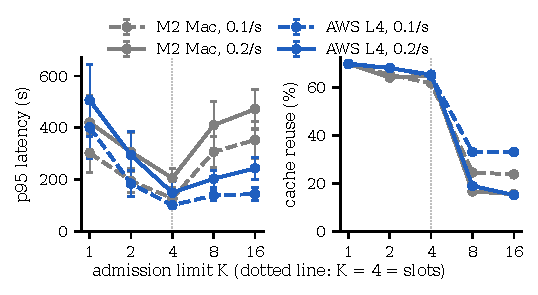
\includegraphics[width=\columnwidth]{fig_ksweep.pdf}
\caption{Phase 1: FIFO with fixed $K$ (short tool calls, mean of 3 seeds). Latency is lowest at $K=4$, the slot count; above it, agents evict each other's context and prompt-cache reuse collapses.}
\label{fig:ksweep}
\end{figure}

\begin{table}[t]
\caption{Phase 1: going from $K=4$ to $K=8$ at 0.2 tasks/s (mean of 3 seeds)}
\label{tab:mech}
\centering\footnotesize
\begin{tabular}{@{}lll@{}}
\toprule
 & M2 Mac & AWS L4-6Q \\
\midrule
Prompt-cache reuse & 65\% $\rightarrow$ 17\% & 65\% $\rightarrow$ 19\% \\
Median prompt time / request & 1.17 $\rightarrow$ 3.55\,s & 0.37 $\rightarrow$ 0.96\,s \\
Generation / request & 12.3 $\rightarrow$ 8.9 tok/s & 12.4 $\rightarrow$ 10.8 tok/s \\
p95 task latency & 205 $\rightarrow$ 410\,s & 149 $\rightarrow$ 203\,s \\
\bottomrule
\end{tabular}
\end{table}

\begin{figure}[t]
\centering
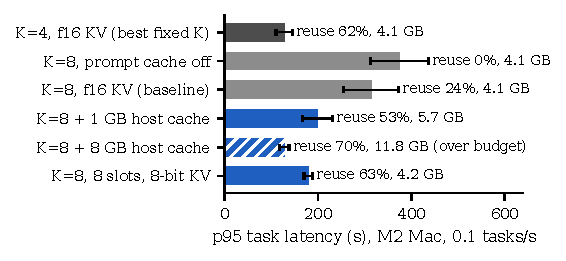
\includegraphics[width=\columnwidth]{fig_retention.pdf}
\caption{Phase 1 causal test: $K=8$ on the M2 Mac at 0.1 tasks/s (mean $\pm$1 std of 3 seeds; memory is weights plus measured footprint). Retaining evicted context recovers latency, but llama.cpp's host-RAM cache needs memory beyond the budget to do so (hatched).}
\label{fig:retention}
\end{figure}

\textbf{Findings.} Fig.~\ref{fig:ksweep} summarizes 90 runs. On both machines the best fixed $K$ equals the slot count. Raising $K$ above it makes every metric worse: from $K=4$ to $K=8$ at 0.2 tasks/s, prompt-cache reuse falls from 65\% to 17--19\% and p95 rises 2.0$\times$ on the Mac but 1.4$\times$ on AWS (Table~\ref{tab:mech}). A returning agent usually finds its slot reassigned and reprocesses its whole history; each request spends 2.4\,s more on prompt processing on the Mac but only 0.6\,s on AWS, and these long recomputations also slow the generation of requests batched with them. A causal test confirmed the cause (Fig.~\ref{fig:retention}): keeping evicted prompts in llama.cpp's host-RAM cache at $K=8$ restored 70\% reuse and the best fixed $K$'s latency, but needed 11.8\,GB; a 1\,GB cache within budget recovered about 60\% of the gap. An 8-bit KV cache fits 8 slots in the memory of 4 with outputs identical to f16 on 50 scored prompts. The penalty for exceeding the slots is the reuse lost times the recomputation cost, which motivated Phase~2: keep agents' context across tool calls without spending the memory budget on it.

\begin{figure*}[t]
\centering
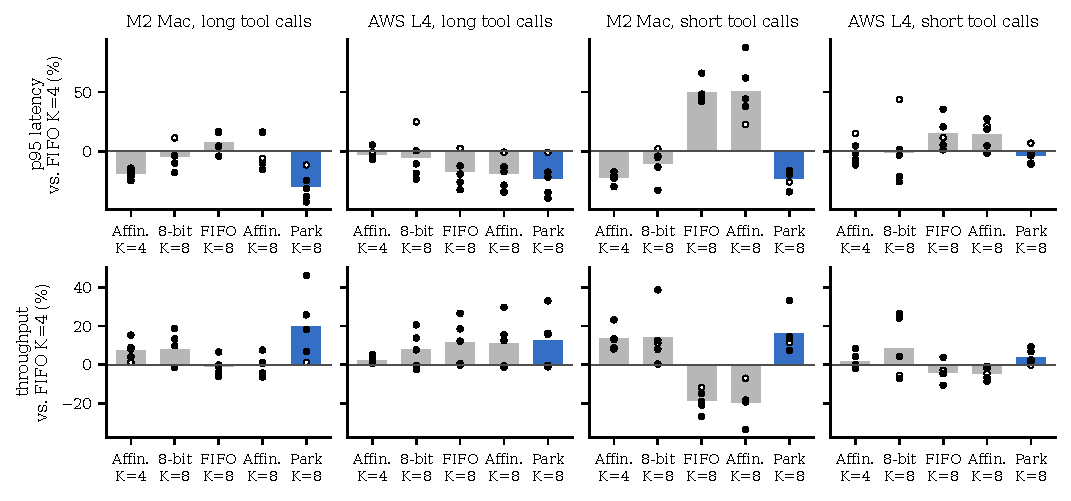
\includegraphics[width=\textwidth]{fig_final.pdf}
\caption{Held-out evaluation: p95 task latency (top) and throughput (bottom) relative to FIFO at $K=4$ with server slot choice, on the same workload seed. Bars: mean of seeds 1000--1002; dots: individual seeds (hollow: seed 1000, light load). Parking at $K=8$ gives the largest gains with long tool calls on both machines and is neutral with short tool calls.}
\label{fig:final}
\end{figure*}

\section{Design}
\begin{figure}[t]
\centering
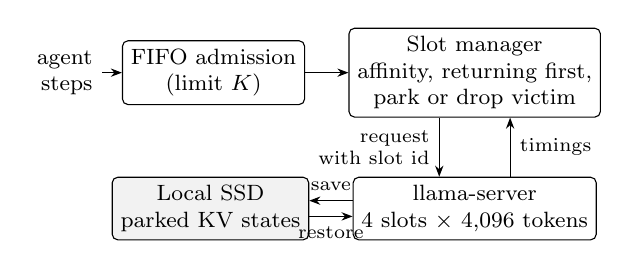
\begin{tikzpicture}[font=\footnotesize, box/.style={draw, rounded corners=2pt, align=center, minimum height=0.62cm, inner sep=3pt}, >={Stealth[length=4pt]}]
\node[box, minimum width=2.1cm] (adm) {FIFO admission\\(limit $K$)};
\node[box, right=0.55cm of adm, minimum width=2.6cm] (mgr) {Slot manager\\affinity, returning first,\\park or drop victim};
\node[box, below=0.75cm of mgr, minimum width=2.6cm] (srv) {llama-server\\4 slots $\times$ 4,096 tokens};
\node[box, left=0.55cm of srv, minimum width=2.1cm, fill=black!5] (ssd) {Local SSD\\parked KV states};
\node[left=0.25cm of adm, align=right] (ag) {agent\\steps};
\draw[->] (ag) -- (adm);
\draw[->] (adm) -- (mgr);
\draw[->] ([xshift=-0.45cm]mgr.south) -- node[left, align=right, font=\scriptsize] {request\\with slot id} ([xshift=-0.45cm]srv.north);
\draw[->] ([xshift=0.45cm]srv.north) -- node[right, font=\scriptsize] {timings} ([xshift=0.45cm]mgr.south);
\draw[->] ([yshift=0.1cm]srv.west) -- node[above, font=\scriptsize] {save} ([yshift=0.1cm]ssd.east);
\draw[->] ([yshift=-0.1cm]ssd.east) -- node[below, font=\scriptsize] {restore} ([yshift=-0.1cm]srv.west);
\end{tikzpicture}
\caption{The slot manager sits in the client between admission and llama-server. It chooses the slot of every request and moves waiting agents' context between slots and the SSD through llama-server's slot save/restore endpoints.}
\label{fig:design}
\end{figure}

\textbf{Overview.} Fig.~\ref{fig:design} shows the design. Admission stays FIFO with a limit $K$, which may now exceed the slot count. A slot manager in the client then decides, for every model call, which slot it runs in and what happens to the context it displaces. It tracks which agent's context is resident in each slot, which slots are busy, and which agents are waiting on a tool. It sends each request with an explicit slot id, so llama-server never chooses a slot on its own.

\textbf{Slot choice.} An agent whose context is resident in an idle slot always gets that slot (\emph{affinity}). Otherwise free slots go first to returning agents, which are partway through a task, and then to new tasks in arrival order. An agent takes an empty slot if one exists; only when every idle slot holds the context of an agent waiting on a tool does it evict one, choosing the least recently used.

\textbf{Parking.} Before evicting, the manager saves the victim slot's KV state to a file on the local SSD (\texttt{POST /slots/\{id\}?action=save}); when the victim returns, it restores the file into a free slot (\texttt{action=restore}) and resumes with its whole history reused. Saving happens only when a slot is actually needed, so agents that keep their slot pay nothing, and a context is never parked twice. Parked files are deleted when they are restored or the task ends. A parked context occupies about 110\,KB per token, so the SSD, not the 6\,GB budget, holds waiting agents.

\textbf{Implementation.} The manager is under 300 lines of asyncio Python in our harness and needs no change to llama.cpp; the server only needs \texttt{--slot-save-path}. It logs every save, restore and drop with its duration and size. On AWS the parked files go to the instance's local NVMe SSD, since the root volume is a small network disk. A mock llama-server with simulated save/restore let us test the pipeline without a model.

\section{Evaluation}
\textbf{Methodology.} We evaluate on held-out seeds 1000--1002 on both machines and two workloads: the Phase~1 mix at 0.2 tasks/s (\emph{short tool calls}, 0.5--4\,s) and the same mix with tool calls of 5--15\,s for short agents and 10--30\,s for long agents at 0.1 tasks/s (\emph{long tool calls}, as for web search or code execution). We compare FIFO at $K=4$ with server slot choice (the Phase~1 baseline); FIFO at $K=4$ with our slot affinity but no parking; FIFO at $K=8$; the best configuration-only baseline from Phase~1, 8 slots with an 8-bit KV cache in the same KV memory; and parking at $K=8$ and 16. Load differs strongly between seeds (seed 1000 is light: every configuration's p95 is below 70\,s), so we compare configurations on the same seed and report per-seed differences.


\subsection{Main results}
Fig.~\ref{fig:final} shows the results; Table~\ref{tab:main} lists absolute values on the two loaded seeds.

\textbf{Long tool calls.} Parking is best on both machines. Against the strongest baseline, FIFO at $K=4$ with affinity, it lowers p95 by 27\% and 8\% on the two loaded seeds on the Mac and by 36\% and 18\% on AWS, and raises throughput by 27\%/8\% and 30\%/13\%. Against the Phase~1 baseline the gains are 22--43\% in p95 and 16--46\% in throughput, and against the 8-bit configuration 21--30\% in p95. With $K=4$, slots sit idle while agents wait on 5--30\,s tools; parking lets $K=8$ fill those gaps without losing context. Without parking, $K=8$ evicts on the Mac and gains nothing; on AWS, where recomputation is 4$\times$ cheaper, plain $K=8$ already recovers part of the benefit (Fig.~\ref{fig:final}). $K=16$ performs like $K=8$.

\textbf{Short tool calls.} Parking is neutral: within $\pm$7\% of FIFO $K=4$ with affinity on every seed and machine. Tool waits are too short for $K=4$ to leave slots idle, so there is little for extra admission to use. The gain over the Phase~1 baseline here (16--19\% p95 on the Mac) comes from affinity, not parking.

\begin{table}[t]
\caption{p95 latency (s) and throughput (tasks/s), mean of the two loaded held-out seeds (1001, 1002)}
\label{tab:main}
\centering\footnotesize\setlength{\tabcolsep}{3.5pt}
\begin{tabular}{@{}lcccc@{}}
\toprule
 & \multicolumn{2}{c}{Long tool calls} & \multicolumn{2}{c}{Short tool calls} \\
 & Mac & AWS & Mac & AWS \\
\midrule
FIFO $K=4$ & 302 / .047 & 271 / .050 & 226 / .075 & 172 / .086 \\
+ affinity, $K=4$ & 241 / .053 & 256 / .051 & 183 / .084 & 156 / .092 \\
8-bit, 8 slots, $K=8$ & 266 / .054 & 235 / .057 & 205 / .082 & 149 / .099 \\
\textbf{Parking, $K=8$} & \textbf{197 / .062} & \textbf{184 / .062} & 186 / .085 & 160 / .091 \\
\bottomrule
\end{tabular}
\end{table}

\textbf{Who benefits.} Short tasks gain most because they no longer queue behind agents that hold slots while waiting on tools: with long tool calls, chat p95 (mean of three seeds) falls from 114 to 28\,s on the Mac and from 89 to 16\,s on AWS (FIFO $K=4$ vs.\ parking). Long agents also improve, from 316 to 204\,s and 288 to 199\,s.

\subsection{Overhead}
Parking cost is small on both machines (Table~\ref{tab:overhead}). A save or restore takes a median of 30--80\,ms against 0.7--9.7\,s to recompute 1,000--3,500 tokens, so restoring is 9--21$\times$ faster than recomputing. All saves and restores together occupy at most 1.7\% of a run's time, which bounds their slowdown of other agents even if they stalled the server completely. Server memory is unchanged: the Mac's footprint rose by under 20\,MB and AWS GPU memory by 2\,MB, while 0.7--1.0\,GB of context sat on the SSD at peak. One caveat is that the operating system's file cache may hold recently written files in RAM; that memory belongs to the OS, not the server, and would be reclaimed under pressure.

\begin{table}[t]
\caption{Parking overhead (held-out runs with parking, $K=8$ and 16)}
\label{tab:overhead}
\centering\footnotesize\setlength{\tabcolsep}{4pt}
\begin{tabular}{@{}lcc@{}}
\toprule
 & M2 Mac & AWS L4 \\
\midrule
Save, median / p95 (ms) & 44--60 / 103--147 & 39--40 / 73 \\
Restore, median / p95 (ms) & 46--78 / 193--200 & 34 / 62--63 \\
Recompute 1k / 3.5k tokens (ms) & 2,599 / 9,660 & 690 / 2,330 \\
Save + restore share of run time & $\le$1.7\% & $\le$1.0\% \\
Peak parked on SSD (GB) & 0.6--1.0 & 0.6--1.0 \\
Server memory vs.\ FIFO $K=4$ & +$<$20\,MB & +2\,MB GPU \\
\bottomrule
\end{tabular}
\end{table}

\subsection{Slot affinity: a flaw in llama.cpp's slot choice}
Even at $K=4$, where every agent could keep its own slot, FIFO with server slot choice lost a returning agent's context in 47--48 of 128 returning steps with long tool calls and 9--21 of 128 with short ones. In every case a free slot existed. llama-server picks the idle slot whose cached prompt shares the longest prefix with the new request, if the shared fraction exceeds 10\%, and otherwise the least recently used. Because all agents share a 200-token system prompt, a new short request matches every slot, including one holding a waiting agent's 2,000-token conversation, and overwrites it. Our manager's affinity rule (prefer empty slots, never take a waiting agent's slot while another is free) removed all of these evictions and alone lowered p95 by 14--21\% on the Mac (less on AWS, where recomputing is cheap). This is a scheduling fix, distinct from parking, and we report the two separately.

\subsection{What did not work}
\textbf{Cost-aware parking.} We built a variant that drops contexts too short to be worth saving and evicts the agent expected to return last, after KVFlow~\cite{pan2025kvflow}. It never differed from plain parking: every evicted context was long enough that parking won, and expected-return order rarely differed from LRU. Since restoring costs at most 0.2\,s per task, there is little for a cost model to decide on our hardware.

\textbf{Restoring early.} Prefetching a context before the tool call ends, as CachedAttention and KVFlow do, could save at most the restore time: 0.15\,s of an 81\,s mean task on the Mac. We did not build it. The remaining delay is waiting for one of the four slots (7--15\,s per task), not data movement.

\textbf{Parking plus 8-bit KV.} Combining parking with 8 slots of 8-bit KV cut slot waiting from 27 to 7\,s on development seeds but raised p95 (Mac 210 to 248\,s): with 8 requests generating at once, each decodes more slowly and long agents finish later. Throughput was unchanged; the accelerator's compute, not memory, became the limit. More slots shift latency from short to long tasks rather than reducing it.

\section{Discussion}
\textbf{When should an edge server park?} Parking pays off when three conditions hold together: more agents are waiting on tools than there are slots, their contexts are long, and the tool calls are long enough that slots would otherwise idle. The first two make eviction frequent and expensive; the third makes extra admission useful. Our short-tool-call workload meets the first two but not the third, so parking only matched the best fixed $K$. Because a save or restore costs tens of milliseconds while recomputation costs seconds, the decision to park, once a slot is needed, is rarely close on our hardware; the real decision is how many agents to admit, and parking makes admitting more of them safe.

\textbf{Hardware.} The two platforms differ 4$\times$ in prompt-processing speed, yet parking helped on both. The difference shows up in the baselines instead: without parking, admitting more agents is harmful on the Mac, where lost context is expensive to rebuild, and nearly free on AWS. A larger model would raise both the recomputation cost and the size of each parked file (KV bytes per token grow with layers and heads), so parking should matter more, not less, as long as the SSD can absorb the traffic; at our scale a run wrote 3--4\,GB on average and at most 7.7\,GB, a modest load for an SSD but one that grows with model size and agent count.

\textbf{Toward the server.} Our manager runs in the client and needs only the existing slot save/restore endpoints, which kept the server untouched but costs a file write per eviction. Inside llama.cpp, the same policy could copy KV blocks to host memory or the SSD asynchronously and fix the slot-selection flaw for all clients; the affinity rule alone is a few lines in the slot chooser.

\section{Experience}
\textbf{What went wrong.} A sweep that we interrupted left its llama-server running on port 8080; the next sweep's servers failed to bind, while the stray one answered every request, so 22 runs silently measured the wrong configuration. We detected it from a slot count that did not match the configuration, discarded and reran the runs, and made the harness refuse a busy port and verify that the answering server is its own. A pilot's memory grew to 7\,GB, which we traced to llama.cpp's default 8\,GB host-RAM prompt cache; we disabled it for budgeted runs and studied it separately. Back-to-back streamed requests failed with ``server disconnected'' because the client reused connections the server had already closed; fresh connections per request fixed it. Our first cache-hit metric counted the whole slot, including the previous answer, rather than reused prompt tokens. Operationally, cloud-synced folders on the Mac reverted edited files several times, and the AWS root disk had 4\,GB free, too little for parked contexts, until we used the instance's NVMe store.

\textbf{What we learned.} Two predictions failed. We expected parking to lose on AWS, where recomputation is cheap and we assumed a network disk; on the local NVMe it was faster than on the Mac. We expected parking to beat the best fixed $K$ on the original workload; it only matched it, which led us to the long-tool-call experiment where it does win. Measuring the ceiling of an idea before building it (restore-early) saved a week. Large load differences between seeds made means with standard deviations misleading, so comparing configurations on the same seed was essential.

\textbf{What worked well.} A mock server for testing the pipeline without a model; a fresh server, fixed output lengths and seeded workloads for every run; resumable sweeps with completion markers, which survived interruptions and a \$3/day cloud budget; logging every request, task, and context movement so that new questions (such as the slot-affinity flaw) could be answered from existing runs; and held-out seeds for the final evaluation.

\section{Limitations and Conclusion}
The workload is synthetic: filler text with chosen tool delays, not traces of real agents. We evaluate one 3B model on llama.cpp's fixed slots; paged servers degrade differently. Three held-out seeds per configuration show consistent direction but not tight confidence intervals, and the Mac's memory budget is enforced by configuration.

On an edge server, agents that wait on tools should not hold their slot's memory, and should not lose their context either. Parking it on the local SSD is cheap, 30--80\,ms per move, and turns idle slots into useful work when tool calls are long, lowering p95 latency by up to 36\% and raising throughput by up to 30\% over the strongest baseline, within the same memory budget. When tool calls are short, a simple slot-affinity rule is enough.

\bibliographystyle{IEEEtran}
\bibliography{refs}

\end{document}
